\documentclass[tikz,border=2pt]{standalone}
\usepackage{tikz}
\usepackage{amsmath}
\usepackage[T1]{fontenc}
\usetikzlibrary{arrows.meta, positioning, calc}

% --- FONT (house invariant — do not remove) ---
\usepackage{helvet}
\renewcommand{\familydefault}{\sfdefault}
\usepackage{sansmath}
\sansmath

% --- COLORS ---
% Recolour of ExoMol_at_10.jpeg into the UCL palette used by the MARVEL figures.
% Original roles: dark slate (theory) -> uclDarkPurple, light teal
% (intermediate surfaces/lines) -> uclLightBlue, orange (experiment) -> uclLightOrange.
\definecolor{uclDarkPurple}{HTML}{361A54}
\definecolor{uclLightBlue}{HTML}{118DFF}
\definecolor{uclLightOrange}{HTML}{E66C37}
\definecolor{flowGrey}{HTML}{9B9B9B}
\definecolor{labelInk}{HTML}{231F20}

% Filled box from (x1,y1) to (x2,y2) with centred label: {fill}{x1}{y1}{x2}{y2}{text}
\newcommand{\ebox}[6]{%
  \fill[#1] (#2,#3) rectangle (#4,#5);
  \node[boxtext] at ($(#2,#3)!0.5!(#4,#5)$) {#6};}

\begin{document}

% Coordinates are pixels of the original 1247x1087 JPEG (y down), 1 px = 0.1 mm.
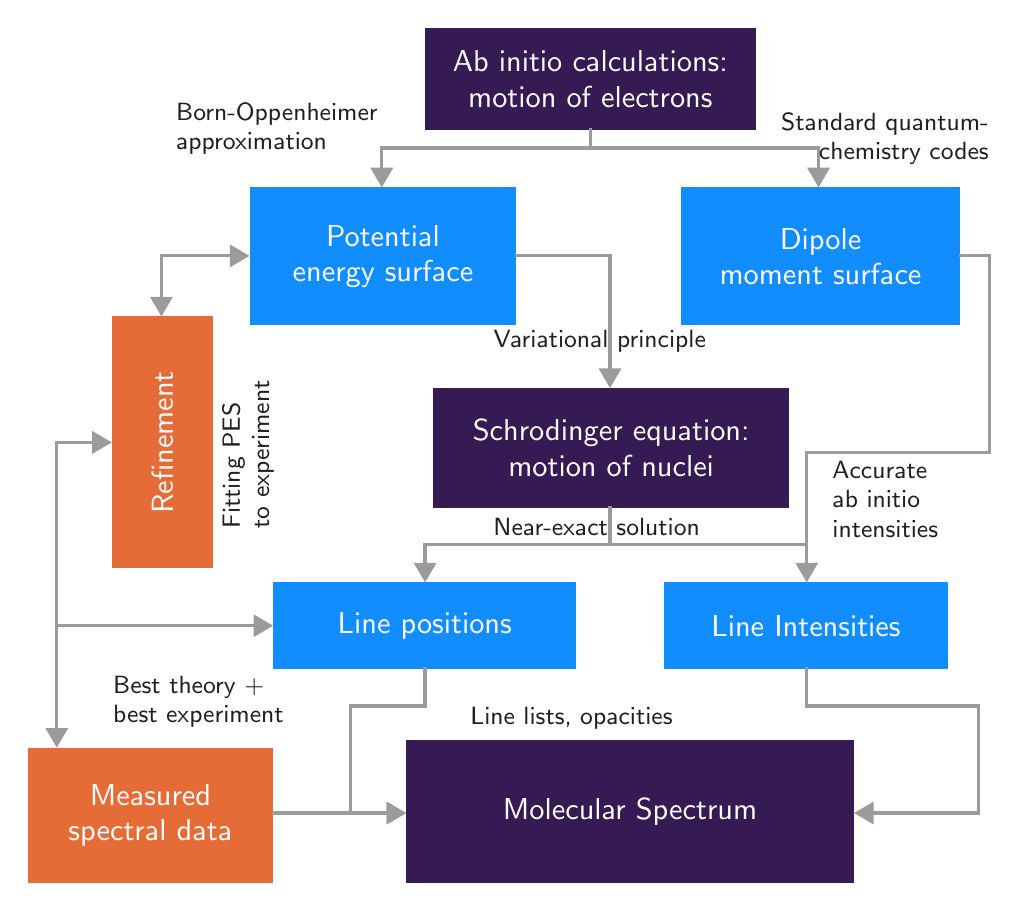
\begin{tikzpicture}[
    x=0.01cm, y=-0.01cm,
    font=\sffamily,
    boxtext/.style={text=white, align=center, inner sep=0pt,
                    font=\fontseries{bc}\fontsize{10.5}{12.8}\selectfont},
    note/.style={text=labelInk, inner sep=0pt,
                 font=\fontseries{mc}\fontshape{it}\fontsize{9}{10.6}\selectfont},
    line/.style={flowGrey, line width=1.15pt, line cap=rect},
    arrow/.style={line, -{Triangle[length=2.5mm, width=2.8mm]}},
    biarrow/.style={line, {Triangle[length=2.5mm, width=2.8mm]}-{Triangle[length=2.5mm, width=2.8mm]}},
]

% --- BOXES ---
\ebox{uclDarkPurple}{505}{0}{925}{130}{Ab initio calculations:\\motion of electrons}
\ebox{uclLightBlue}{282}{203}{621}{378}{Potential\\energy surface}
\ebox{uclLightBlue}{830}{203}{1185}{378}{Dipole\\moment surface}
\fill[uclLightOrange] (107,367) rectangle (235,687);
\node[boxtext, rotate=90] at (171,527) {Refinement};
\ebox{uclDarkPurple}{515}{458}{968}{610}{Schrodinger equation:\\motion of nuclei}
\ebox{uclLightBlue}{312}{705}{697}{815}{Line positions}
\ebox{uclLightBlue}{808}{705}{1170}{815}{Line Intensities}
\ebox{uclLightOrange}{0}{915}{312}{1087}{Measured\\spectral data}
\ebox{uclDarkPurple}{481}{905}{1050}{1087}{Molecular Spectrum}

% --- FLOW ---
\draw[line]  (715,130) -- (715,153);
\draw[arrow] (715,153) -| (450,203);
\draw[arrow] (715,153) -| (1005,203);
\draw[arrow] (621,290) -| (740,458);
\draw[arrow] (1185,290) -| (1222,540) -| (990,705);
\draw[line]  (740,610) -- (740,657) -- (990,657);
\draw[arrow] (740,657) -| (505,705);
\draw[arrow] (505,815) |- (410,862) |- (481,998);
\draw[arrow] (312,998) -- (481,998);
\draw[arrow] (990,815) |- (1208,862) |- (1050,998);
\draw[biarrow] (170,367) |- (282,290);
\draw[arrow] (37,527) -- (37,915);
\draw[arrow] (37,527) -- (107,527);
\draw[arrow] (37,760) -- (312,760);

% --- ANNOTATIONS ---
\node[note, align=left,  anchor=north west] at (188,95)  {Born-Oppenheimer\\approximation};
\node[note, align=right, anchor=north east] at (1222,108) {Standard quantum-\\chemistry codes};
\node[note] at (727,398) {Variational principle};
\node[note, align=left, rotate=90, anchor=north west] at (247,637) {Fitting PES\\to experiment};
\node[note, align=left,  anchor=north west] at (1022,550) {Accurate\\ab initio\\intensities};
\node[note] at (723,634) {Near-exact solution};
\node[note, align=left,  anchor=north west] at (108,823) {Best theory +\\best experiment};
\node[note] at (691,877) {Line lists, opacities};

\end{tikzpicture}

\end{document}
